\subsection{Intégration avec PHP et Laravel} % (fold)
\label{sub:integration_avec_php_et_laravel}

	MongoDB bénéficie d'une extension PHP facilement installable via PEAR (le gestionnaire d'extensions de PHP). Deux limitations existent néanmoins : le support de la version 3.0 de MongoDB n'est pas encore pris en charge et l'extension n'est pas encore compatible avec la toute dernière version majeure de PHP (PHP 7.0) prévue pour fin novembre. La mise à jour de l'extension vers la toute dernière version de MongoDB et de PHP sera sans doute effective rapidement.\\

	Afin de faciliter le développement, il a été décidé d'utiliser un ORM. Dans le cas des bases de données orientées documents, nous allons utiliser un ODM pour Object Document Mapping. Plusieurs grands ORM existent dans le monde des frameworks PHP : Doctrine et Eloquent sont deux des plus connus. Tous deux proposent un ODM associé. Doctrine présente l'avantage de permettre une intégration de MongoDB via un package PHP officiel. Eloquent supporte le système de base de données MongoDB via un package non-officiel (développé par jenssegers) appelé tout simplement \verb|mongodb|. Dans les deux cas, l'outil permet de gérer toutes les opérations de base ainsi que les documents imbriqués. Nous avons décidé d'utiliser Laravel et donc son ORM officiel Eloquent, nous allons donc utiliser le package \verb|jenssegers/mongodb| dans sa version 2.0.\\

	L'utilisation d'une base de données NoSQL est souvent délicate car il en existe de nombreux types différents et les intégrations ne sont donc pas forcément toutes développées (et rarement intégrée par des packages officiels). Il est donc préférable de se limiter aux bases de données les plus utilisées pour chaque type (MongoDB pour les bases de données orientées documents, Redis pour les bases de données orientées clé / valeur par exemple.). Dans notre cas, MongoDB étant très utilisée, il existe donc de nombreuses intégrations, comme nous l'avons vu pour PHP, mais aussi pour les différents ORM du marché ainsi que pour la plupart des solutions de test de l'écosystème (nous ne détaillerons pas les solutions de test dans ce rapport).

% subsection integration_avec_php_et_laravel (end)

\section{Modélisation} % (fold)
\label{sec:modelisation}

	Comme expliqué dans notre introduction aux bases de données orientées documents, il n'existe pas de schéma fixe pour ces dernières. Pour autant, lors du développement d'une vraie application, il est nécessaire pour les développeurs de se fixer des schémas afin de pouvoir utiliser la base de données.\\

	Nous avons organisé notre base de données en 4 collections : \verb|recipes|, \verb|locations|, \verb|guests| et \verb|events|.

	\subsection{Diagramme de stockage}

		\begin{figure}[H]
			\centering
			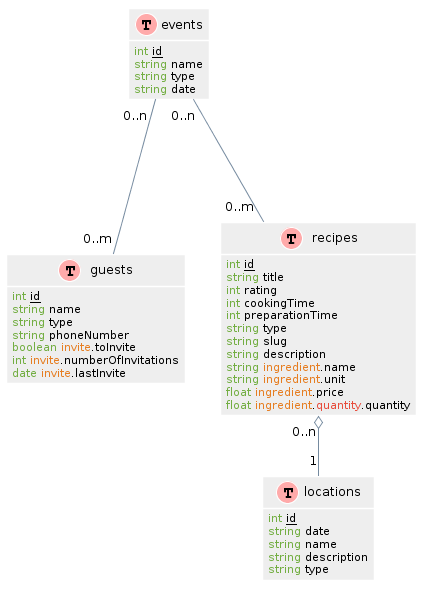
\includegraphics[width=0.5\textwidth]{images/diagramme-stockage.png}
			\caption{Diagramme de stockage de l'application dans une base de données orientée documents.}
			\label{fig:diagramme-stockage}
		\end{figure}

		Le diagramme de stockage de notre application est présenté dans la figure~\ref{fig:diagramme-stockage}. Les clés primaires de chaque collection sont soulignées. Les documents imbriqués sont représentés par des variations de couleurs dans les champs d'une collection. Les champs supplémentaires nécessaires aux relations \enquote{plusieurs vers plusieurs} ne sont pas représentés.

	\subsection{Recettes et ingrédients}

		Les recettes sont stockées dans la collection \verb|recipes|. Il n'existe pas de collection pour les ingrédients et leur quantité associée car nous avons décidé d'utiliser l'imbrication de documents afin de les stocker directement dans chaque recette.

		\paragraph{Avantage de la solution} % (fold)
		 \label{par:avantage_de_la_solution}
		 	Lors de la récupération de chaque recette, les ingrédients sont automatiquement récupérés. Nous savons que dans la majorité des cas les informations sur les ingrédients seront nécessaire à l'affichage d'une recette, cette solution présente donc un avantage au niveau des performances (un seul document est à récupérer pour afficher une recette avec ses ingrédients). De plus, dans le cas présent, les ingrédients sont très succints (nom, unité, quantité et prix) et chaque recette ne possède que peu d'ingrédients donc cette solution ne va pas surcharger notre document parent.
		 % paragraph avantage_de_la_solution (end)

		 \paragraph{Désavantage de la solution} % (fold)
		 \label{par:desavantage_de_la_solution}
		 	Avec cette approche, il est très coûteux de récupérer la liste de tous les ingrédients car il faut parcourir toutes les recettes. De plus, cette solution nous oblige à dupliquer des informations pour chaque recette ayant des ingrédients identiques. Mettre à jour un ingrédient spécifique nous obligera à modifier indépendamment chaque recette utilisant cet ingrédient.
		 % paragraph desavantage_de_la_solution (end)

		 \paragraph{Avantages contre désavantages} % (fold)
		 \label{par:avantages_contre_desavantages}
		 	Dans notre application, le cas d'utilisation le plus utilisé sera l'affichage de recette. Il est donc préférable d'optimiser les lectures via l'imbrication. La possibilité de mettre à jour les ingrédients n'est pas prévue et dans le cas où elle serait ajoutée, elle resterait très rare par rapport à l'affichage. Le coût de mise à jour n'est donc pas un problème.
		 % paragraph avantages_contre_desavantages (end)

% section modelisation (end)